\chapter{Experiments}
\label{Chapter5}

This chapter is organized in sections corresponding to each of the extensions we've outlined in section \ref{sec:ch1.objective}. For each extension we provide a general description of the idea with the rationale behind it, a brief complexity analysis, a pseudocode, and a detailed analysis of the experimental results.

The first section of this chapter does not correspond to any extension and is instead an introductory block.

\section{Introduction}

\subsection{General Framework}

\texttt{Sklearn}, being a general machine learning library, has its own implementation of the base \texttt{RFE} algorithm. Given that it is open source, we were able to base our own implementation on it. After pruning the code to its bare minimum (no dep\-en\-den\-cies), we began to add our own extensions. We organized each extension in its own folder, isolated from the rest, and copied the base implementation there.

For the actual experiments we've used \texttt{Jupiter Notebooks} (integrated in \texttt{Visual Studio Code}). Each experiment may use different notebooks depending on what is being tested exactly. Some code that is common to all notebooks, such a code for plotting, has been placed at the beginning (for convenience). The implementation of SVM-RFE and associated usability methods has been moved to separate Python files. This is both a convenient software pattern and a requirement of the parallelization library on Windows.

We use \emph{k-fold cross-validation} to perform the experiments multiple times with different folds, as explained in section \ref{sec:ch4.performance}. For the same experiment, the same amount of folds is used, but different amounts may be used in different experiments. We've parallelized this procedure with the standard \texttt{multiprocessing.pool} library. Given that our CPU has 8 cores, for the most computationally expensive experiments we're using 6 or 7-fold cross-validation in order to be able to finish the experiment in a single round (with one or two spare cores to be able to keep working in the machine). The execution time is always calculated as the mean of the elapsed times in every SVM-RFE execution (single core).

A limitation of Python parallelization when using Jupiter is that standard output gets suppressed. In order to debug (since debugging tools also don't work in this context) we raised exceptions, which are not suppressed because they reach the main thread. In some situations we've used other methods such a file logging or temporally running the code without parallelization.

For plotting we've used the \texttt{Mathplotlib} library. We have made a custom plot function that includes all relevant information for SVM-RFE. Having a standard plot design allows for easy comparison as shown in Figure \ref{fig:ch4.tradeoff}. This plot displays the accuracy (vertical axis) of each feature subset (by size, horizontal axis) selected by the SVM-RFE algorithm. We calculate and display both the train accuracy and the test accuracy (which is that of the va\-lid\-ation set when cross-validation is used). We also show where the optimal is based on the linear scalarization method. Furthermore, we also show what the minimum accuracy is, based on the amount of classes, with a doted red horizontal line. And finally we show with an overlay scatter plot of small vertical lines what the actual feature selection subset sizes where and what accuracy they had during the execution of SVM-RFE (training accuracy). It is important not to confuse this plot with plots describing an iterative optimization process or model selection.

\subsection{The data}

\subsubsection*{Sklearn Generator}

The general machine learning library \texttt{Sklearn} provides tools to generate artificial datasets for various prob\-lems. We're using the \texttt{make\_classification} gen\-er\-a\-tor, which creates normally-distributed clus\-ters of points placed at the vertices of an hypercube. Multiple clusters can corresponding to a single class. This specific gen\-er\-a\-tor also introduces in\-ter\-de\-pen\-dence between features and var\-i\-ous types of noise.

We've selected this generator because it allows to specify the amount of in\-for\-ma\-tive (i.e. non-redundant, useful) features the dataset should have, it can generate multi-class datasets, and by changing the amount of clusters per class it can control the separability of the data.

We don't use a single dataset of this kind in our experiments. Instead, we use datasets generated with the parameters that we think can better help evaluate the expected properties and correctness of the extensions.

\subsubsection*{MADELON}
\label{sec:ch5.data.madelon}

This is one of the five datasets proposed for the NIPS (Neural Information Processing Systems) 2003 challenge in feature selection. The dataset remains publicly available in the UCI (University of California, Irvine) machine learning repository. The results of this challenge can be found at the workshop web page (\cite{guyon_result_2004}).

The winner of the challenge got an accuracy of 92.89\% with 8 selected features. However, this is using test data that is not publicly available. Using only the avail\-able data we've found articles describing the use of this dataset where the maximum accuracy reached is 88\%. 

This dataset is constructed similarly to the \texttt{sklearn} \texttt{make\_classification} gen\-er\-a\-tor. It uses clusters of points placed at the vertices of some hypercube, however, instead of a single hypercube it uses five of them. Also, this method labels each in hypercube in one of two classes randomly. Five features correspond to the which hypercube a point is in, with an extra 15 being redundant features extracted from linear combinations of the first 5. The total amount of features per data point is 500, 480 of them being noise (also called probes).

Of this dataset, 2000 observations are publicly available and where used in this project, 600 are part of a separate validation set not used in this project, and 1800 are part of a test set not used in this project and also not publicly available. All sets have the same amount of positive and negative samples.

\subsubsection*{Digits}

For the multi-class classification extension we've used the digits dataset (Optical Recognition of Handwritten Digits Data Set). This is also a dataset available in the UCI machine learning repository and is also provided ready to use in \texttt{Sklearn}. This dataset contains 5620 instances of 64 features corresponding to 10 possible handwritten digits. Each feature has been extracted from a 32×32 bitmap by count\-ing the pixels of 4×4 non-overlapping blocks. There are 64 informative features.

For this dataset common accuracy results are around 98\%, but we've found some cases where it can reach 100\%.

\begin{table}
    \centering
    \begin{tabular}{l c c c c}
    \toprule
    \tabhead{Name}      & \tabhead{Observations} & \tabhead{Features} & \tabhead{Informative}& \tabhead{Classes} \\
    \midrule
    \texttt{make\_classification}   & - & - & - & - \\
    MADELON                         & 2000 & 500 & 5 & 2 \\
    Digits                          & 1797 & 64 & ?? & 10 \\
    \bottomrule\\
    \end{tabular}
    \caption{Summary of dataset properties.}
    \label{tab:ch5.datasetdesc}
\end{table}

% -----------------------------------------------------------------------------------------

\section{Dynamic Step}

This extension is based on the constant step variant of SVM-RFE (Algorithm \ref{alg:rfe1}), however, instead of using some constant number $t$ as the step in each iteration, we calculate that number dynamically. The most straightforward way to do this is by using a percentage.

\subsection{Description and reasoning}
\label{sec:dynamicStep.desc}

The percentage is a hyper-parameter. It is used within every iteration to eliminate a number of the least ranked features. A constant step has already been used in pract\-ice, but it is expected that this method will be significantly faster without effecting the accuracy performance, or even improving it.

Other similar modifications are also found in the literature, including using the square root of the remaining features \texttt{SQRT-RFE}, an entropy based function \texttt{E-RFE}, or \texttt{RFE-Annealing} which sets the step at $|\vt{s}| \frac{1}{i+1}$, thus, changing the percentage each iteration (\cite{ding_improving_2006}).

\iffalse
That is, the amount of features eliminated "$r$" at $j$-th iteration is the summation of the amount of features eliminated each iteration, i.e. $np^i$:

\begin{equation}\label{eq:dynamicStep1}
    r = \sum_{i = 1}^{j}{(np^i)} 
\end{equation}

It may be more interesting to see complexity as in the amount of iterations re\-quired to eliminate $r$ features, it can be derived from equation \ref{eq:dynamicStep1} as follows:

\begin{align*}
    r &= n \sum_{i = 1}^{j}{p^i} = n \sum_{i = 0}^{j-1}{(p^i)} - n + np^j \\
    \frac{r}{n} &= \frac{1-p^j}{1-p} - 1 + p^j \\
    \frac{r}{n} &= \frac{(1-p^j) - (1-p) + (1-p)p^j}{1-p}\\
    \frac{(1-p)r}{n} &= (1-p^j) - (1-p) + (p^j-p^{j+1})\\
    \frac{(1-p)r}{n} &= 1 -p^j -1 + p + p^j - p^{j+1}\\
    \frac{(1-p)r}{n} &= p - p^{j+1}\\
    - \frac{(1-p)r}{n} + p &= p^{j+1}\\
    \log_{p} \left( - \frac{(1-p)r - np}{n} \right) &= \log_{p} (p^{j+1})\\
    \log_{p} \left( - \frac{(1-p)r - np}{n} \right) &= j + 1\\
    \log_{1/p} \left( - \frac{n}{(1-p)r} + 1/p \right) &= j + 1\\
\end{align*}
\fi

We assume that, the bigger the step each iteration, the worse the performance of the ranking. This is consistent with what we've seen in figure \ref{fig:ch4.dynamicStep.vanilla.comp}. However, since we're eliminating the worst variables first, eliminating more of them at once shouldn't affect performance because it is likely they would've been eliminated in the next iterations anyway. The fewer the iterations remaining, the riskier it becomes to eliminate multiple variables at once, and thus a smaller step is beneficial.

\subsubsection*{Our expectations for this extension are:}

\begin{itemize}
    \item \textbf{Improvement in time complexity:} Given that SVM complexity $O(dn^2)$ is lin\-ear\-ly dependent on the amount of dimensions $d$, we know that each iteration is faster than the one before it. By increasing the step in the first iterations we should drastically reduce the time it takes to complete, even if then we decide to reduce the step in later, less time-consuming, iterations.
    \item \textbf{Improvement in accuracy performance:} Using dynamic step, compared to a constant step $t > 1$, can also improve the accuracy. This is because the last iterations may be performed with a step $t \ge i \ge 1$.
\end{itemize}

Note that by adjusting the percentage you can decide for which of these two objectives you want to optimize, it may also be possible to find a middle case in which both the accuracy and the time are improved.

\subsection{Pseudocode formalization}

\begin{algorithm}[H]
    \DontPrintSemicolon
      \KwInput{$p$ \tcp*{p = percentage, $0 \le p \le 1$}}
      \KwOutput{$\vt{r}$}
      \KwData{$X_0,\vt{y}$}
      $\vt{s} = [1,2, \dotsc, d]$ \tcp*{subset of surviving features}
      $\vt{r} = []$ \tcp*{feature ranking list} 
      \While{$|\vt{s}| > 0$}
        {
            \tcc*[h]{Restrict training examples to good feature indices}\\
            $X=X_0(:,\vt{s})$\VS

            \tcc*[h]{Train the classifier}\\
            $\vt{\alpha} = \texttt{SVM-train(} X, y \texttt{)}$\VS

            \tcc*[h]{Compute the weight vector of dimension length $|\vt{s}|$}\\
            $\vt{w} = \sum_k{\vt{\alpha_k} \vt{y_k} \vt{x_k}}$\VS

            \tcc*[h]{Compute the ranking criteria}\\
            $\vt{c} = [(w_i)^2 \text{ for all $i$}]$\VS

            \tcc*[h]{Compute $t$ based on the percentage}\\
            $t = p|\vt{s}|$\VS

            \tcc*[h]{Find the $t$ features with the smallest ranking criterion}\\
            $\vt{f} = \texttt{argsort}(\vt{c})(\ :t)$\VS

            \tcc*[h]{Iterate over the feature subset}\\
            \For{$f_i \in \vt{f}$}{
                \tcc*[h]{Update the feature ranking list}\\
                $\vt{r} = [\vt{s}(f_i), ...\vt{r}]$\VS
    
                \tcc*[h]{Eliminate the feature selected}\\
                $\vt{s} = [...\vt{s}(1:f_i - 1), ...\vt{s}(f_i + 1:|\vt{s}|)]$
            }
        }
    \caption{SVM-RFE with DynamicStep}
\end{algorithm}
\VS
Note that since we do a non-lineal skip focused on the iterations that take more time we can achieve a reduced complexity of $O(\log(d)dn^2)$. This can be illustrated in Figure \ref{fig:ch5.dstep.comparetime}, where we show the relationship between the amount of remaining features and iterations for the different step methods. 

\begin{figure}[h]
    \centering
    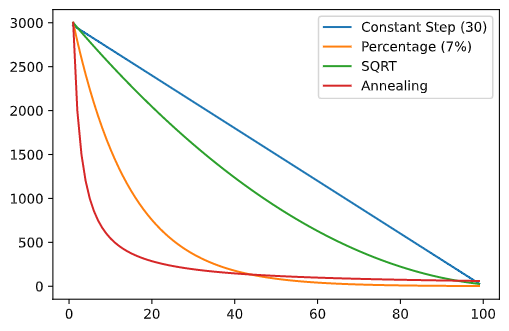
\includegraphics[width=0.4\linewidth]{img/ch5/comparetimes.png}
    \caption{Amount of features remaining (vertical axis) at each iteration (horizontal axis).}
    \label{fig:ch5.dstep.comparetime}
\end{figure}

The relative time cost of each method can be estimated as the area under the curve. Note that in this plot the amount of iterations is fixed, however in practice it may make more sense that dynamic step methods perform much more late iterations than constant step.

\subsection{Results}

\subsubsection*{Analysis with artificially generated data}

We generate a 2 class dataset with the following code. The scalarization trade-off used is of 80\% accuracy, 20\% feature subset size. All results are mean values extracted from a 7-fold cross-validation procedure.

\begin{verbatim}
    X, y = make_classification(
        n_samples = 1000, n_clusters_per_class=3, n_features = 300,
        n_informative = 100, n_redundant=100, n_repeated=20,
        flip_y=0.05, random_state=2, class_sep=2
    )
\end{verbatim}

We start by comparing how the dataset performs under a random feature se\-lec\-tion or a simple filter method. For the validation phase a linear SVM has been used, with the regularization parameter found by grid search and being $C = 0.00001$.

\begin{figure}[H]
    \centering
    \begin{subfigure}[b]{0.4\linewidth}
        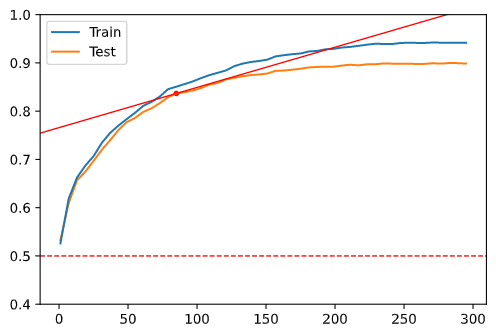
\includegraphics[width=\linewidth]{img/ch5/dstep/random.png}
        \subcaption*{Random AT (85, 0.83, 0.187)}
    \end{subfigure}
    \begin{subfigure}[b]{0.4\linewidth}
        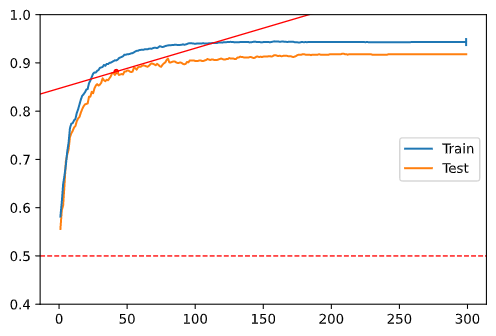
\includegraphics[width=\linewidth]{img/ch5/dstep/filter.png}
        \subcaption*{Filter AT (42, 0.88, 0.122)}
    \end{subfigure}
    \caption{Accuracy of feature rankings produced either by a random method or an SVM-based filter method. AT (\emph{feat.}, \emph{acc.}, \emph{cost})}
    \label{fig:ch5.dstep.init}
\end{figure}

Based on these results we expect that SVM-RFE must perform better than the filter method. Or objective now is to find if using a dynamic step can perform similarly or better than SVM-RFE in less amount of time. From a grid search model selection procedure we'be selected the best feature rankings, shown in Figure \ref{fig:ch5.dstep.vanillabest}.

\begin{figure}[H]
    \centering
    \begin{subfigure}[b]{0.4\linewidth}
        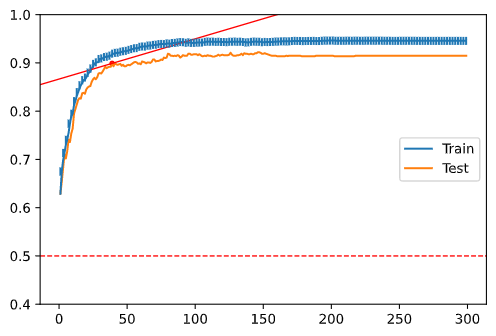
\includegraphics[width=\linewidth]{img/ch5/dstep/vanilla1.png}
        \subcaption*{Const Step $t=2, C=0.00001$}
    \end{subfigure}
    \begin{subfigure}[b]{0.4\linewidth}
        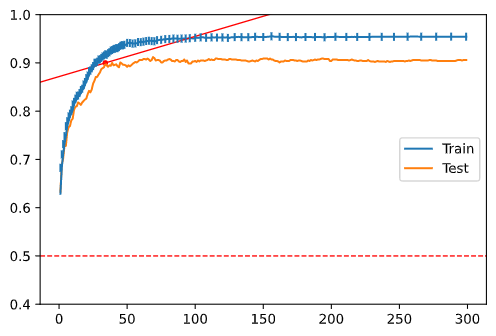
\includegraphics[width=\linewidth]{img/ch5/dstep/vanilla2.png}
        \subcaption*{Dynamic Step $p=0.05, C=0.0001$}
    \end{subfigure}
    \caption{Accuracy of the best feature rankings produced by SVM-RFE with constant or dynamic step.}
    \label{fig:ch5.dstep.vanillabest}
\end{figure}

In the following tables we detail the results of the model selection. The cell corresponding to the best model of each algorithm (by cost) and associated time have been highlighted. 
\begin{table}[H]
    \centering
    \begin{tabular}{l | c c c|c c c|c c c}
        \toprule
        \multicolumn{1}{c}{Step} & \multicolumn{3}{c}{\textbf{2}} & \multicolumn{3}{c}{\textbf{10}} & \multicolumn{3}{c}{\textbf{50}}\\
        %\cline{2-4}\cline{5-7}\cline{8-10}
        \midrule
        \textbf{$C$}&Feat.&Acc.&Cost&Feat.&Acc.&Cost&Feat.&Acc.&Cost \\
        \midrule
        \textbf{0.000001} &    39 & 88.40\% & 0.119 &    41 & 89.40\% & 0.112 &    38 & 88.70\% & 0.116\\
        \textbf{0.000010} &    \mrk{39} & \mrk{89.90\%} & \mrk{0.107} &    57 & 90.70\% & 0.112 &    54 & 89.80\% & 0.118\\
        \textbf{0.000100} &    55 & 91.00\% & 0.109 &    61 & 91.30\% & 0.110 &    59 & 90.10\% & 0.118\\
        \textbf{0.001000} &    81 & 89.40\% & 0.139 &    77 & 87.90\% & 0.148 &    81 & 87.10\% & 0.157\\
        \textbf{0.010000} &   104 & 88.70\% & 0.160 &   103 & 89.10\% & 0.156 &   116 & 87.90\% & 0.174\\
        \bottomrule
        \end{tabular}
    \caption{Grid search of SVM-RFE with constant step.}
\end{table}

\begin{table}[H]
    \centering
    \begin{tabular}{l | c c c}
        \toprule
        \multicolumn{1}{c}{\textbf{C/Step}} & \textbf{2} & \textbf{10} & \textbf{50} \\
        %\cline{2-4}\cline{5-7}\cline{8-10}
        \midrule
        \textbf{0.000001} & 0:03.691 & 0:00.643 & 0:00.124\\
        \textbf{0.000010} & \mrk{0:05.242} & 0:01.050 & 0:00.190\\
        \textbf{0.000100} & 0:07.001 & 0:01.440 & 0:00.279\\
        \textbf{0.001000} & 0:08.039 & 0:01.522 & 0:00.334\\
        \textbf{0.010000} & 0:11.834 & 0:02.424 & 0:00.577\\
        \bottomrule
        \end{tabular}
    \caption{Execution time (min:sec.msec) of SVM-RFE with constant step.}
\end{table}

\begin{table}[H]
    \centering
    \begin{tabular}{l | c c c|c c c|c c c}
        \toprule
        \multicolumn{1}{c}{Percentage} & \multicolumn{3}{c}{\textbf{0.04}} & \multicolumn{3}{c}{\textbf{0.12}} & \multicolumn{3}{c}{\textbf{0.20}}\\
        %\cline{2-4}\cline{5-7}\cline{8-10}
        \midrule
        \textbf{$C$}&Feat.&Acc.&Cost&Feat.&Acc.&Cost&Feat.&Acc.&Cost \\
        \midrule
        \textbf{0.000001} &    26 & 88.20\% & 0.112 &    22 & 86.60\% & 0.122 &    37 & 88.10\% & 0.120\\
        \textbf{0.000010} &    43 & 89.80\% & 0.110 &    36 & 89.80\% & 0.106 &    60 & 89.30\% & 0.126\\
        \textbf{0.000100} &    \mrk{34} & \mrk{90.00\%} & \mrk{0.103} &    59 & 91.00\% & 0.111 &    42 & 90.40\% & 0.105\\
        \textbf{0.001000} &    56 & 87.30\% & 0.139 &    63 & 87.20\% & 0.144 &    91 & 89.00\% & 0.149\\
        \textbf{0.010000} &    87 & 88.40\% & 0.151 &   104 & 87.40\% & 0.170 &   107 & 87.90\% & 0.168\\
        \bottomrule
        \end{tabular}
    \caption{Grid search of SVM-RFE with dynamic step.}
\end{table}

\begin{table}[H]
    \centering
    \begin{tabular}{l | c c c}
        \toprule
        \multicolumn{1}{c}{\textbf{C/Percentage}} & \textbf{0.04} & \textbf{0.12} & \textbf{0.20} \\
        %\cline{2-4}\cline{5-7}\cline{8-10}
        \midrule
        \textbf{0.000001} & 0:01.048 & 0:00.324 & 0:00.202\\
        \textbf{0.000010} & 0:01.455 & 0:00.443 & 0:00.283\\
        \textbf{0.000100} & \mrk{0:01.947} & 0:00.612 & 0:00.380\\
        \textbf{0.001000} & 0:02.505 & 0:00.709 & 0:00.404\\
        \textbf{0.010000} & 0:03.487 & 0:01.079 & 0:00.639\\
        \bottomrule
        \end{tabular}
    \caption{Execution time (min:sec.msec) of SVM-RFE with dynamic step.}
\end{table}

Note that the three best models for dynamic step are all better than the best model using constant step. This results however have to be taken with a grain of salt, given that variance is present and the difference is only marginal.

A more clear-cut improvement can be seen on the computational cost, which had a speedup of x2.7 even when the model used by dynamic step had a greater value of $C$. (Equation \ref{eq:ch5.dstep.speedup1}).
\label{eq:ch5.dstep.speedup1}
\begin{align}
    \text{Speedup} = \frac{T_{\text{old}}}{T_{\text{new}}} = \frac{5.242}{1.947} = 2.692
\end{align}

\begin{verbatim}
    NOTE: The speedup is better the highier the amount of features.
\end{verbatim}


\subsubsection*{Analysis with Madelon}

Like before, we start comparing how the dataset performs under a random ranking (Figure \ref{fig:ch5.dstep.madelon.rand}).

\begin{figure}[H]
    \centering
    \begin{subfigure}[b]{0.4\linewidth}
        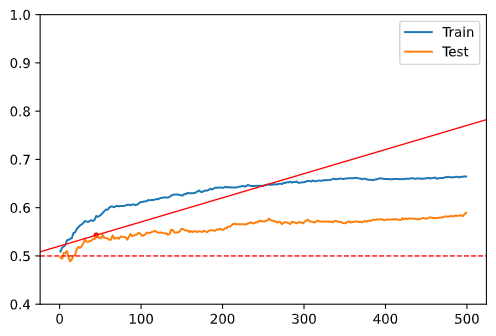
\includegraphics[width=\linewidth]{img/ch5/dstep/madelon-random.png}
        \subcaption*{$C=10^{-5}$}
    \end{subfigure}
    \begin{subfigure}[b]{0.4\linewidth}
        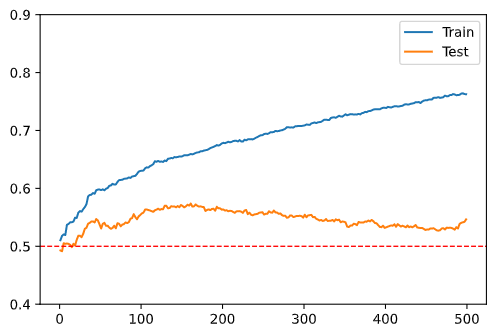
\includegraphics[width=\linewidth]{img/ch5/madelon-random-c_1}
        \subcaption*{$C=10^3$}
    \end{subfigure}
    \caption{Accuracy of an SVM classifier with a random feature selection with the Madelon dataset.}
    \label{fig:ch5.dstep.madelon.rand}
\end{figure}

It seems to perform poorly, even when all features are used. We thought this could be caused by the regularization parameter, so we tried various values of $C$ on a logarithmic scale (Figure \ref{fig:ch5.dstep.madelon.reg}). At first glance, however, it doesn't look like a regularization problem.

\begin{figure}[h]
    \centering
    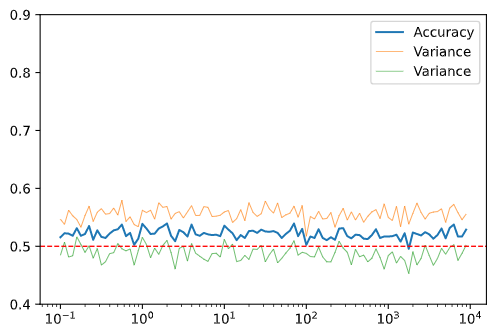
\includegraphics[width=0.4\linewidth]{img/ch5/madelon-cv-c}
    \caption{Hyper-parameter search of $C$. Displaying test accuracy of a linear SVM classifier using all features.}
    \label{fig:ch5.dstep.madelon.reg}
\end{figure}

Next've we've tried to see what happens if we apply normal SVM-RFE directly, with $C=10^{-6}$, see Figure \ref{fig:ch5.dstep.madelon.lin}. Unfortunately, not only is the accuracy much lower than expected (Section \ref{sec:ch5.data.madelon}), but also no improvement can be appreciated when we decrease the step. This indicates that dynamic step will not work, as it relies on this property.

\begin{figure}[h]
    \centering
    \begin{subfigure}[b]{0.4\linewidth}
        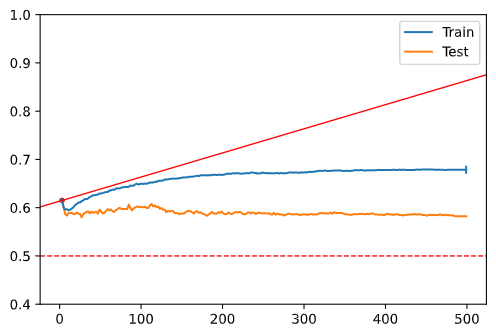
\includegraphics[width=\linewidth]{img/ch5/dstep/madelon-lin1.png}
        \subcaption*{Filter}
    \end{subfigure}
    \begin{subfigure}[b]{0.4\linewidth}
        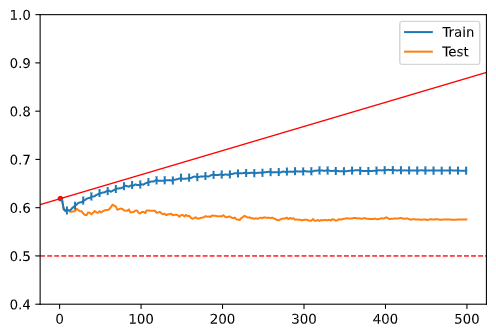
\includegraphics[width=\linewidth]{img/ch5/dstep/madelon-lin2.png}
        \subcaption*{Step = 10}
    \end{subfigure}
    \caption{Accuracy of the ranking produced by SVM-RFE.}
    \label{fig:ch5.dstep.madelon.lin}
\end{figure}

Since the problem is not regularization, then it may be that the data is not linearly separable. Although we can not implement a non-linear kernel for the SVM-RFE procedure yet (it is another extension), we may be able to improve the situation by using a non-lineal kernel on the validation phase.

\begin{figure}[h]
    \centering
    \begin{subfigure}[b]{0.4\linewidth}
        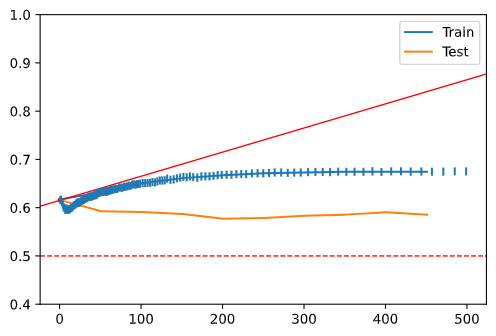
\includegraphics[width=\linewidth]{img/ch5/dstep/madelon-dyn1.png}
        \subcaption*{Lineal, $C = 10^{-6}$}
    \end{subfigure}
    \begin{subfigure}[b]{0.4\linewidth}
        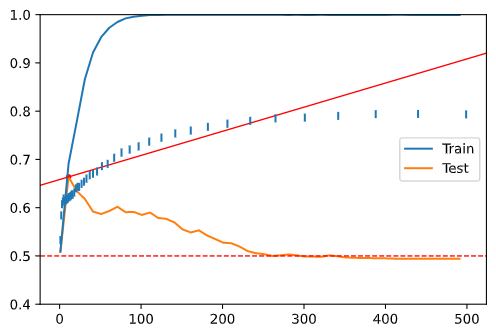
\includegraphics[width=\linewidth]{img/ch5/dstep/madelon-dyn2.png}
        \subcaption*{Polynomial, degree 6, $C = 0.6$}
    \end{subfigure}
    \caption{Accuracy of the ranking produced by a dynamic step SVM-RFE with lineal and polynomial kernels.}
    \label{fig:ch5.dstep.madelon.dyn}
\end{figure}

As expected, dynamic step doesn't improve the accuracy in this scenario. We do see an improvement when using a non-lineal kernel on the validation phase, but again produces the same result as the filter method.

\subsection{Conclusions}

This is a summary of the pros and cons that we've found for this extension:

\begin{itemize}
    \item Using some form of dynamic step may improve the accuracy in certain sce\-nar\-ios, specially in situations where there is a benefit from having a small step.
    \item Using a percentage doesn't introduce a new hyper-parameter since it replaces the existing step constant.
    \item Dynamic step is generally much faster than a constant step for the same levels of accuracy, specially when many features are used and the step is small.
    \item With independence of the accuracy improvement, dynamic step can still be used to speed up considerably the validation phase.
    \item The percentage and final point are better adjusted when the shape of the data is known.
\end{itemize}

In general, we recommend using dynamic step whenever possible, after the initial exploration of the data and if possible after the execution with the associated filter method.

% -----------------------------------------------------------------------------------------

\section{Sampling}

\section{Stop Condition}

% -----------------------------------------------------------------------------------------

\section{Multi-Class}

In this section we extend SVM-RFE to the multi-class classification problem.

\subsection{Description and reasoning}
\label{sec:stopCond.desc}

When it comes to extending SVM to handle a multi-class problems two common methods exists, OvR (One-vs-Rest) and OvO (One-vs-One). In both cases the idea is to divide the problem in a set of binary classification problems and use a joint decision function that operates on the results of each of these. Because we're not really making any predictions during the SVM-RFE procedure, we can not use this joint decision function. Instead, we must find a way to merge the ranking criteria obtained form each problem to find a joint ranking criteria.

We know that the ranking criteria is an estimator of the importance of some feature for a given binary decision problem. It can be the case that a feature is very useful to distinguish between two classes but useless for the rest. In this case a joint ranking criteria formed by taking the mean, the median or the sum will result in poor selections. A better idea would be to take the maximum. However, it may also be desirable to estimate the joint importance a feature has by considering its individual importance in more than one problem, that is, a feature that is important in more than one binary classification problem is more important than another that is only important in one such classification problem even if the second feature has a greater individual importance. A way to perform such ranking would be, for instance, the sum of the squares. For both methods proposed a normalization of all feature rankings is probably adequate.

Note that \texttt{sklearn} only supports OvO, and is therefore the option we will use.

\subsection{Pseudocode formalization}

\textbf{Definitions:}

\begin{itemize}
    \item $X_0 = [\vt{x_0}, \vt{x_1}, \dotsc, \vt{x_k}]^T$ list of observations.
    \item $\vt{y} = [y_1, y_2, \dotsc, y_k]^T$ list of labels.
\end{itemize}

\begin{algorithm}[H]
    \DontPrintSemicolon
      \KwInput{$t$ \tcp*{$t$ = step}}
      \KwOutput{$\vt{r}$}
      \KwData{$X_0,\vt{y}$}
      $\vt{s} = [1,2, \dotsc, n]$ \tcp*{subset of surviving features}
      $\vt{r} = []$ \tcp*{feature ranked list}
      \While{$|\vt{s}| > 0$}
        {
            \tcc*[h]{Restrict training examples to good feature indices}\\
            $X=X_0(:,\vt{s})$\VS

            \tcc*[h]{Compute the joint ranking criteria}\\
            $\vt{c} = [0, 0, \dots, ]$\\
            \For{$\vt{Xl} \subseteq \vt{X}$, $\vt{yl} \subseteq \vt{y}$ with $\vt{Xl}$ and $\vt{yl}$ being an instance of OvO}{
                \tcc*[h]{Train the classifier}\\
                $\vt{\alpha} = \texttt{SVM-train(} \vt{Xl}, \vt{yl} \texttt{)}$\VS

                \tcc*[h]{Compute the weight vector of dimension length $|\vt{s}|$}\\
                $\vt{w} = \sum_k{\vt{\alpha_k} \vt{yl_k} \vt{Xl_k}}$\VS
    
                \tcc*[h]{Compute the joint ranking criteria}\\
                $\vt{c} = [\max(c_i, (w_i)^2) \text{ for all $i$}]$\VS
            }\VS

            \tcc*[h]{Find the $t$ features with the smallest ranking criterion}\\
            $\vt{f} = \texttt{argsort}(\vt{c})(\ :t)$\VS

            \tcc*[h]{Iterate over the feature subset}\\
            \For{$f_i \in \vt{f}$}{
                \tcc*[h]{Update the feature ranking list}\\
                $\vt{r} = [\vt{s}(f_i), ...\vt{r}]$\VS
    
                \tcc*[h]{Eliminate the feature selected}\\
                $\vt{s} = [...\vt{s}(1:f_i - 1), ...\vt{s}(f_i + 1:|\vt{s}|)]$
            }
        }
    \caption{SVM-RFE for multi-class classification problems}
    \label{alg:svmrfe-stopcond}
\end{algorithm}

\subsection{Results}

\section{Non-linear Kernels}

\section{Combo}


----

In this section 

\begin{itemize}
    \item Importance of scaling preprocessing
    \item Complexity analysis and pseudocode.
\end{itemize}